% File was used for presenting, it includes more breaks and pauses

%----------------------------------------------------------------------------------------
%	%PACKAGES, THEMES and COMMANDS
%----------------------------------------------------------------------------------------
\documentclass[aspectratio=169,xcolor=dvipsnames]{beamer}

\usetheme{Boadilla}

\usecolortheme{dolphin}
\setbeamertemplate{caption}[numbered]
\usepackage{amsmath}
\usepackage{mathtools}
\usepackage{tikz}

\DeclareMathOperator{\R}{\mathbb{R}}
\newcommand{\blue}{\color{myblue}}
\newcommand{\red}{\color{red}}
\newcommand{\green}{\color{ForestGreen}}
\newcommand{\black}{\color{black}}
\newcommand{\di}{\text{d}}
\definecolor{myblue}{RGB}{60,60,200}
%----------------------------------------------------------------------------------------
%	TITLE PAGE
%----------------------------------------------------------------------------------------

\title[BNP models for bipartite graphs, F. Caron]{Bayesian nonparametric models for bipartite graphs
} \subtitle{François Caron}
\author[Andrea Teruzzi] {Andrea Teruzzi}
\date[20605 - Machine Learning II]{September 5, 2022} 


%----------------------------------------------------------------------------------------
%	INTRODUCTION SLIDES
%----------------------------------------------------------------------------------------

\begin{document}
\begin{frame}
    \titlepage
\end{frame}
%----------------------------------------------------

\AtBeginSection[]
{
  \begin{frame}
    \frametitle{Table of Contents}
    \tableofcontents[currentsection,hideothersubsections,currentsubsection]
  \end{frame}
}

%----------------------------------------------------------------------------------------
%	PRESENTATION SLIDES
%----------------------------------------------------------------------------------------

%------------------------------------------------
\section{Bipartite Networks} %going beyond IBP and stable IBP
%------------------------------------------------
\begin{frame}{Bipartite Networks}
\begin{block}{Definition}
    A \textbf{bipartite graph} is a graph $g=(V, E)$, where vertices $V$ are divided in two sets $A$ and $B$ and edges $E$ can occur only between elements of two different sets.
    \vspace{5pt}
\end{block}
\pause
Real world examples:
\begin{itemize}
    \item Scientists authoring papers
    \item Internet users posting messages on forums
    \item \textbf{Readers reading books}
\end{itemize}
\pause
\begin{block}{Definition}
    We say \textbf{degree of a vertex} the number of edges connected to that vertex.
    \vspace{5pt}
\end{block}

\end{frame}
%------------------------------------------------
\begin{frame}{Bipartite Networks} 

\begin{center}
    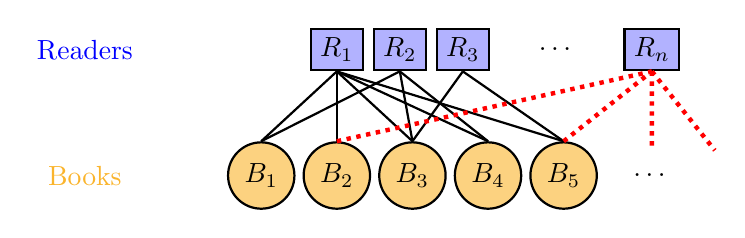
\begin{tikzpicture}[scale = 1.6] \vspace{-0.5cm}
        %style
        \tikzset{circle/.style = {shape=circle, draw ,minimum size=1.5em, fill=Dandelion, fill opacity=0.6, text opacity=1, thick}}
        \tikzset{square/.style = {shape=rectangle, draw, minimum size=1.5em,fill = blue, fill opacity=0.3, text opacity=1, thick}}
        \tikzset{circle_n/.style = {shape=circle, draw=red ,minimum size=1.5em, fill=Dandelion, fill opacity=0.6, text opacity=1, very thick}}
        \tikzset{square_n/.style = {shape=rectangle, draw=black ,minimum size=1.5em,fill = blue, fill opacity=0.3, text opacity=1,  thick}}
        \tikzset{edge/.style = {thick}}
        \tikzset{edge_n/.style = {draw=red, ultra thick, dotted}}

        % slide 2
        \onslide<2->{
        \node[blue] at (-2,0) {Readers};
        \node[square] (B1) at  (0,0) {$R_1$};
        \node[square] (B2) at  (0.5,0) {$R_2$};
        \node[square] (B3) at  (1,0) {$R_3$};

        \node[Dandelion] at (-2,-1) {Books};
        \node[circle] (R1) at  (-0.6,-1) {$B_1$};
        \node[circle] (R2) at  (0,-1) {$B_2$};
        \node[circle] (R3) at  (0.6,-1) {$B_3$};
        \node[circle] (R4) at  (1.2,-1) {$B_4$};
        \node[circle] (R5) at  (1.8,-1) {$B_5$};

        \draw[edge] (R1.north) to (B1.south);
        \draw[edge] (R1.north) to (B2.south);
        \draw[edge] (R2.north) to (B1.south);
        \draw[edge] (R3.north) to (B1.south);
        \draw[edge] (R3.north) to (B2.south);
        \draw[edge] (R3.north) to (B3.south);
        \draw[edge] (R4.north) to (B1.south);
        \draw[edge] (R4.north) to (B2.south);
        \draw[edge] (R5.north) to (B1.south);
        \draw[edge] (R5.north) to (B3.south);
        }
        %slide 3
        \onslide<3->{
        \node[square_n] (B4) at  (2.5,0) {$R_n$};
        \node (dots) at (1.75,0) {\ldots};

        \onslide<2->{\node (dots_2) at (2.5,-1) {\ldots};}

        \draw[edge_n] (R2.north) to (B4.south);
        \draw[edge_n] (R5.north) to (B4.south);
        \draw[edge_n] (B4.south) to (2.5,-0.8);
        \draw[edge_n] (B4.south) to (3,-0.8);
        } 
    \end{tikzpicture} 
    \end{center}
\vspace{5pt}
\onslide<4->{\textbf{Bayesian nonparametric (BNP)} models for network growth:}
    \begin{itemize}
        \item<5-> Parameter of interest is \textbf{infinite-dimensiona}l (i.e. infinite number of books)
        \item<6-> Bayesian nonparametric (BNP) models:
        \begin{itemize}
            \item<7->  Indian Buffet Process (IBP), but does \underline{not induce power-law behaviour}
            \item<8->  Stable IBP, but \underline{induces Poissonian distribution for the degree of readers}
        \end{itemize}
        \item<9-> Flexible BNP model able to capture \textbf{power-law behaviour} for both books and readers, while retaining \textbf{computational tractability}
    \end{itemize}

\end{frame}
%------------------------------------------------
\section{Statistical model}
%------------------------------------------------
\begin{frame}[t]{Bayesian Model}{Bipartite graph}
\setlength{\leftmargini}{0.2cm}
\begin{itemize}
    \item<2-> We represent a bipartite graph using a collection of atomic measure $ \blue \boldsymbol{Z_{i}}$. For each reader $i = 1, \dots, n$ with books $j = 1, \dots, \infty$:
    $$
    Z_{i} = \sum^{\infty}_{j=1} z_{ij} \delta_{\theta_{j}}
    $$
    where $\blue \boldsymbol{\{\theta\}} \subset \boldsymbol{\Theta}$ the set of books and $\blue \boldsymbol{z_{ij}}$ equal 1 if reader $i$ has read book $j$, 0 otherwise.
   
    \item<3-> For each reader we consider the latent process $\blue \boldsymbol{V_{i}}$:
    $$
    V_{i} = \sum^{\infty}_{j=1} v_{ij} \delta_{\theta_{j}}
    $$
    where $ \blue \boldsymbol{v_{ij}}$ (\underline{inversely}) controls the \textbf{probability of the existence of the edge} between reader $i$ and book $j$.
\end{itemize}


\end{frame}
%------------------------------------------------
\begin{frame}{Bayesian Model}{Latent process}
\setlength{\leftmargini}{0.2cm}

\begin{itemize}
    \item<2-> Assuming:
    $$  
    v_{ij} | \, w_{j}  \sim Exp(w_{j} \gamma_{i})
    $$
    \vspace{-12pt}
    \begin{itemize}
        \item<3-> A positive \textbf{popularity parameter} $\blue \boldsymbol{w_j}$ assigned to each book
        \item<4-> A positive \textbf{interest-in-reading parameter} $\blue \boldsymbol{\gamma_i}$ assigned to each reader
    \end{itemize}
    \vspace{5pt}
    \item<5-> Then, the probability that reader $i$ reads book $j$ is: 
    $$
    p(z_{ij}=1 | w_{j}, \gamma_{i}) = 1 - exp( w_{j} \gamma_{i})
    $$
    
    \onslide<6->{For tractability issues, we consider $\blue \boldsymbol{u_{ij} = \min(v_{ij},1)}$ and the process $\blue \boldsymbol{U_{i}}$. $Z_i$ can be obtained deterministically from $U_i$.}
\end{itemize}


\end{frame}
%------------------------------------------------
\begin{frame}{Bayesian Model}{Book popularity parameter}

\begin{block}<2->{Definition}
    Let $\Theta$ be a measurable space. A \textbf{completely random measure} (\textbf{CRM}) is a random measure G such that for any collection of disjoint measurable subsets $A_1 , \dots , A_n$ of $\Theta$, the random masses of the subsets $G(A_1 ), \dots, G(A_n)$ are independent.
\end{block}
\onslide<3->{$\blue \boldsymbol{\textbf{G} \sim \textbf{CRM}(\lambda, h)}$ with Levy measure: 
$$\Lambda(\di w,\di \theta)=\lambda(w)h(\theta)\di w \di \theta$$}
\onslide<4->{
\hspace{-3pt} Realizations of G take the form of Poisson processes over $\{(w_j , \theta_j ),\, j = 1, \dots, \infty\} \subset \R_{+} \times \Theta$:
$$
G = \sum^{\infty}_{j=1} w_{j} \delta_{\theta_{j}}
$$}
 
\end{frame}
%------------------------------------------------
\begin{frame}{Bayesian Model}{Book popularity parameter}
\onslide<2->{An example of CRM is the \textbf{generalized gamma process} (GGP), which includes the gamma process (GP), the inverse Gaussian process (IGP) and stable process as special cases:
$$
\lambda(w; \, \alpha,\sigma,\tau )= \frac{\alpha}{\Gamma(1-\sigma)}w^{-\sigma-1}e^{-w\tau}
$$
}
\onslide<3->{
\hspace{-10pt} G is an \textbf{homogeneous CRM}:}
\begin{itemize}
    \item<4-> Atoms i.i.d from $h$ (base density), independently from masses
    \item<5-> Masses distributed according to Poisson process over $\R^{+}$ with intensity $\lambda$ (Levy intensity)
\end{itemize}
\onslide<6->{
We assume:
\begin{gather*}
\begin{dcases}
     \int_{0}^{\infty} \lambda(w)\di w = \infty \\
     \int_{0}^{\infty} (1 - e^{-w})\lambda(w)\di w < \infty
\end{dcases}
     \onslide<7->{\Rightarrow \blue \textbf{G}\boldsymbol{(\Theta)}  \color{black} = \sum_{j=1}^{\infty}w_j \textbf{ finite and positive}}
\end{gather*}}

\end{frame}
%------------------------------------------------
\begin{frame}{Bayesian Model}{Hierarchical model}
$\boldsymbol{Z_{i}}$ \textbf{is a Poisson process}, obtained from transformations of Poisson processes.
\begin{block}<2->{Proposition}
    $Z_i$ is marginally characterized by a Poisson process. Furthermore, \textbf{the total mass} $Z_{i}(\Theta) = \sum_{j=1}^{\infty}z_{ij}$, which corresponds to the total number of books read by reader i, \textbf{is finite with probability one and admits a Poisson}$\boldsymbol{(\psi_{\lambda}(\gamma_{i}))}$ \textbf{distribution}, with:
    $$
    \psi_{\lambda}(\gamma_{i}) = \int_{0}^{\infty} (1 - e^{-\gamma_{i}w})\lambda(w)\di w 
    $$
\end{block}
\onslide<3->{
We can sum up the model in the following hierarchical form:
\begin{align*}
     v_{ij}|\, G &\sim \text{Exp}(w_{j} \gamma_{i})\\
     G &\sim \text{CRM}(\lambda, h)
 \end{align*}}
\end{frame}
%------------------------------------------------
\begin{frame}{Bayesian Model}{Posterior Characterization}
\onslide<+->{We observe a set of edges $\{z_{ij}\}$ of a bipartite network
$Z_1,\dots, Z_n$ of n reader:} 
\begin{itemize}[<+->]
    \item $\blue \boldsymbol{K}$ books $\{\theta_1, \dots , \theta_K\}$
    \item $\blue \boldsymbol{K_{i}}\color{black} = Z_i(\Theta) = \sum_{j=1}^{\infty}z_{ij}$ \textbf{the degree of reader} $\boldsymbol{i}$
    \item $\blue \boldsymbol{m_j} \color{black} = \sum_{i=1}^{n}Z(\{\theta_j\})= \sum_{i=1}^{n}z_{ij}$ \textbf{the degree of book} $\boldsymbol{j}$
\end{itemize}
\vspace{10pt}
\onslide<+->{
\textbf{Posterior distribution of the CRM given the latent process $\boldsymbol{U}$} coincides with the distribution of another \red CRM having a rescaled intensity \black and \green fixed observed points of discontinuity \black :
$$
\textbf{G} = \red \boldsymbol{\textbf{G}^{*}} \color{black} \black + \green \sum_{j=1}^{K}w_{j} \delta_{\theta_{j}}
$$}
\end{frame}
%------------------------------------------------
\begin{frame}{Bayesian Model}{Posterior Characterization}
\setlength{\leftmargini}{0.2cm}
\begin{itemize}[<+->]
    \item $\text{G}^{*}$ and $\{w_j\}$ are mutually independent with:
    $$
    \text{G}^{*} \sim \text{CRM}(\lambda^{*}, h) \quad \text{ and } \quad \lambda^{*}(w) = \lambda(w) \exp(-w\sum_{i=1}^{n}\gamma_{i})
    $$
    and the masses:
    $$
    p(w_{j}| \, \text{rest}) \propto \lambda(w_{j}) w_{j}^{m_{j}} \exp(-w_{j} \sum_{i=1}^{n}\gamma_{i}U_{ij})
    $$
    
    \item For the GGP, $ G^{*}$ is still a GGP with parameters $\alpha^{*}=\alpha,\, \sigma^{*}= \sigma \text{ and } \tau^{*} = \tau +\sum_i^{n}\gamma_{i}$ and:
    $$
    w_{j}| \, \text{rest} \sim \text{Gamma}(m_{j} - \sigma, \tau + \sum_{i=1}^{n}\gamma_i u_{ij} )
    $$
\end{itemize}
\end{frame}
%------------------------------------------------
\begin{frame}{Generative Process}
Distribution of $Z_{n}| U_{1}, \dots, U_{n-1}$, with $\blue \boldsymbol{x_{ij}}\black =-\log(u_{ij})$ positive latent score 
\begin{center} 
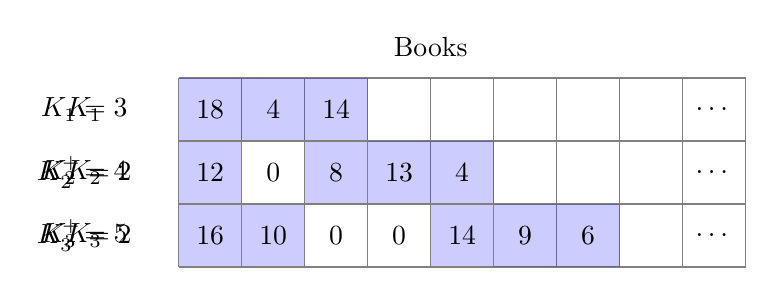
\begin{tikzpicture} [scale = 1.6] 
    %group0
    \onslide<2->{
    \node at (+1.00,+0.75) {Books};
    }
    \onslide<2>{\node at (-1.75,+0.25) {$ K_1$};}
    %group1 
    \onslide<3->{
    \draw[step=0.5cm,color=gray] (-1.00,+0.50) grid (+3.5,+0.00);
    \node at (+3.25,+0.25) {$\dots$};
    \node at (-1.75,+0.25) {$K_1=3$};
    \fill[blue, opacity=0.2] (-1.00,+0.50) rectangle (-0.50,+0.00);
    \fill[blue, opacity=0.2] (-0.50,+0.50) rectangle (+0.00,+0.00);
    \fill[blue, opacity=0.2] (+0.00,+0.50) rectangle (+0.50,+0.00);
    }
    %group2
    \onslide<4->{
    \node at (-0.75,+0.25) {18};
    \node at (-0.25,+0.25) {4};
    \node at (+0.25,+0.25) {14};
    }
    %group3
    \onslide<5-6>{
    \node at (-1.75,-0.25) {$K_{2}$};
    }
    %group4
    \onslide<6>{\draw[step=0.5cm,color=gray] (-1.00,+0.00) grid (+0.5,-0.50);}
    \onslide<6->{
    \fill[blue, opacity=0.2] (-1.00,+0.00) rectangle (-0.50,-0.50);
    \fill[blue, opacity=0.2] (+0.00,+0.00) rectangle (+0.50,-0.50);
    }
    %group5
    \onslide<7>{\node at (-1.75,-0.25) {$K^{+}_2=2$};}
    \onslide<7->{
    \draw[step=0.5cm,color=gray] (-1.00,+0.00) grid (+3.5,-0.50);
    \node at (+3.25,-0.25) {$\dots$};
    \fill[blue, opacity=0.2] (+0.50,+0.00) rectangle (+1.00,-0.50);
    \fill[blue, opacity=0.2] (+1.00,+0.00) rectangle (+1.50,-0.50);
    }
    %group6
    \onslide<8->{
    \node at (-1.75,-0.25) {$K_2=4$};
    \node at (-0.75,-0.25) {12};
    \node at (-0.25,-0.25) {0};
    \node at (+0.25,-0.25) {8};
    \node at (+0.75,-0.25) {13};
    \node at (+1.25,-0.25) {4};
    }
    %group7
    \onslide<9-10>{
    \node at (-1.75,-0.75) {$K_3$};
    }
    %group8
    \onslide<10>{\draw[step=0.5cm,color=gray] (-1.00,-0.50) grid (+1.50,-1.00);}
    \onslide<10->{
    \fill[blue, opacity=0.2] (-1.00,-0.50) rectangle (-0.50,-1.00);
    \fill[blue, opacity=0.2] (-0.50,-0.50) rectangle (+0.00,-1.00);
    \fill[blue, opacity=0.2] (+1.00,-0.50) rectangle (+1.50,-1.00);
    }
    %group9
    \onslide<11>{\node at (-1.75,-0.75) {$K^{+}_3=2$};}
    \onslide<11->{
    \draw[step=0.5cm,color=gray] (-1.00,-0.50) grid (+3.5,-1.00);
    \node at (+3.25,-0.75) {$\dots$};
    \fill[blue, opacity=0.2] (+1.50,-0.50) rectangle (+2.00,-1.00);   
    \fill[blue, opacity=0.2] (+2.00,-0.50) rectangle (+2.50,-1.00);
    }
    %group10
    \onslide<12->{
    \node at (-1.75,-0.75) {$K_3=5$};
    \node at (-0.75,-0.75) {16};
    \node at (-0.25,-0.75) {10};
    \node at (+0.25,-0.75) {0};
    \node at (+0.75,-0.75) {0};
    \node at (+1.25,-0.75) {14};
    \node at (+1.75,-0.75) {9};
    \node at (+2.25,-0.75) {6};
    }
\end{tikzpicture}

\vspace{25pt}
    
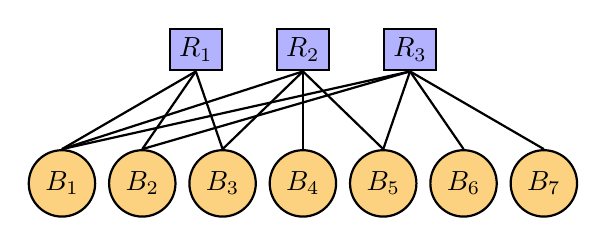
\begin{tikzpicture}[scale = 1.7] 
        %style
        \tikzset{circle/.style = {shape=circle, draw ,minimum size=1.5em, fill=Dandelion, fill opacity=0.6, text opacity=1, thick}}
        \tikzset{square/.style = {shape=rectangle, draw, minimum size=1.5em,fill = blue, fill opacity=0.3, text opacity=1, thick}}
        \tikzset{edge/.style = {thick}}

        %group0
        \onslide<2->{
        \node[square] (R1) at  (+0.40,+0.00) {$R_1$};
        }
        %group1
        \onslide<3->{
        \node[circle] (B1) at  (-0.60,-1.00) {$B_1$};
        \node[circle] (B2) at  (+0.00,-1.00) {$B_2$};
        \node[circle] (B3) at  (+0.60,-1.00) {$B_3$};
        \draw[edge] (R1.south) to (B1.north);
        \draw[edge] (R1.south) to (B2.north);
        \draw[edge] (R1.south) to (B3.north);
        }
        %group2
        
        %group3
        \onslide<5->{
        \node[square] (R2) at  (+1.20,+0.00) {$R_2$};
        }
        %group4
        \onslide<6->{
        \draw[edge] (R2.south) to (B1.north);
        \draw[edge] (R2.south) to (B3.north);
        }
        %group5
        \onslide<7->{
        \node[circle] (B4) at  (+1.20,-1.00) {$B_4$};
        \node[circle] (B5) at  (+1.80,-1.00) {$B_5$};
        \draw[edge] (R2.south) to (B4.north);
        \draw[edge] (R2.south) to (B5.north);
        }
        %group6
        
        %group7
        \onslide<9->{
        \node[square] (R3) at  (+2.00,+0.00) {$R_3$};
        }
        %group8
        \onslide<10->{ 
        \draw[edge] (R3.south) to (B1.north);
        \draw[edge] (R3.south) to (B2.north);
        \draw[edge] (R3.south) to (B5.north);
        }
        %group9
        \onslide<11->{
        \node[circle] (B6) at  (+2.40,-1.00) {$B_6$};
        \node[circle] (B7) at  (+3.00,-1.00) {$B_7$};
        \draw[edge] (R3.south) to (B6.north);
        \draw[edge] (R3.south) to (B7.north);
        }
        %group8
        
\end{tikzpicture}
\end{center}
\end{frame}
%------------------------------------------------
\begin{frame}{Gibbs sampling}
\onslide<+->{We use Gibbs sampler to derive the posterior distribution of $\boldsymbol{U, G | \, Z}$.  \\}
\vspace{5pt}
\onslide<+->{\underline{For the GGP}:}
\begin{enumerate}[<+->]
    \item For $i= 1, \dots, n$ and $j= 1, \dots, K$ set $u_{ij}=1$ if $z_{ij}=0$, otherwise:
    $$
    u_{ij}| \, z_{ij}, w_{j}, \gamma_i \sim \text{rExp}(\gamma_{i} w_{j},1)
    $$
    \item For $j= 1, \dots, K$:
    $$ %popularity parameters of observed books
    w_{j}| U, \gamma_{i} \sim \text{Gamma}(m_{j} - \sigma, \tau + \sum_{i}^{n}\gamma_i u_{ij} ) 
    $$
    and
    $$ %sum of popularity parameters of observed books
    G^{*}(\Theta) \sim \text{Exponentially tilted stable}\footnotemark
    $$
    \end{enumerate}
    \only<4->{\footnotetext[1]{For general cases $G^{*}(\Theta)$ follows $ g^{*}(w)\propto g(w)\exp^{-w\sum_{i}^{n}\gamma_i}  \text{ with } g(w) \text{ the distribution of } G(\Theta)$
    \vspace{7pt}}}
\end{frame}
%------------------------------------------------
%------------------------------------------------
\section{Update of hyperparameters}
\begin{frame}{Update of $\gamma_{i}$}
\begin{enumerate}[<+->]
    \item \textbf{Parametric}: $\gamma_{i}$ to be unknown and estimate them from the graph by assigning a prior $\gamma_{i} \sim \text{Gamma}(a_{\gamma}, \, b_{\gamma})$ and update:
    $$
    \gamma_{i}| \, G, U \sim \text{Gamma}\Big(a_{\gamma}+ \sum_{j}^{K}z_{ij}, \, b_{\gamma}+\sum_{j}^{K}w_{j}u_{ij}+G^{*}(\Theta)\Big)
    $$
    \onslide<+->{But $Z_{i}(\Theta)$ still have a (but more flexible) Poisson distribution!\\ }
    
    \item \textbf{Nonparametric}: Let $\blue \boldsymbol{\Gamma \sim \textbf{CRM}(\lambda_{\gamma}, h_{\gamma})}$ and a measurable space of readers $\blue \boldsymbol{\Tilde{\Theta}}$, which we can represent in the form $\Gamma = \sum^{\infty}_{i=1} \gamma_{i} \delta_{\theta_{j}}$. Conditionally on $(U, w, G^{*}(\Theta))$, we update:
    $$
    \Gamma = \Gamma^{*} + \sum^{n}_{i=1} \gamma_{i} \delta_{\tilde{\theta_{i}}}
    $$
   \onslide<+->{We have more of flexibility in the modelling of the distribution of the degree of readers(\textbf{power-law behavior})!}
\end{enumerate}



\end{frame}
%------------------------------------------------
\begin{frame}{Posterior characterization for GGP for $w_{i}$ and $\gamma_{i}$}
\vspace{5pt}
\onslide<+->{
Let $G$ and $\Gamma$ GGP distributed with parameters $(\alpha, \sigma, \tau)$ and $(\alpha_{\gamma}, \sigma_{\gamma}, \tau_{\gamma})$:}
\vspace{5pt}
\begin{itemize}[<+->]
    \item \underline{Reader update}:  $\Gamma = \Gamma^{*} + \sum^{n}_{i=1} \gamma_{i} \delta_{\tilde{\theta_{i}}}$ with:
    \begin{gather*}
    \Gamma^{*} \sim \text{CRM}(\lambda^{*}_{\gamma}, h_{\gamma}) \\
    \gamma_{i} | \, U,G \sim \text{Gamma}\big(K_{i}- \sigma_{\gamma}, \tau_{\gamma} + \sum_{j=1}^{K} w_{j}u_{ij} + G^{*}(\Theta)\big)     
    \end{gather*}

    \item \underline{Book update}: $G = G^{*} + \sum^{K}_{i=1} w_{i} \delta_{\theta_{i}}$ with:
    \begin{gather*}
     G^{*} \sim \text{CRM}(\lambda^{*}, h) \\
     w_{i} | \, U, \Gamma \sim \text{Gamma}\big(m_{j}- \sigma, \tau + \sum_{i=1}^{n} \gamma_{i}u_{ij} + \Gamma^{*}(\Tilde{\Theta})\big)
    \end{gather*}
\end{itemize}

\end{frame}
%------------------------------------------------
\section{Power-law properties and real-world examples}
\begin{frame}{Power-law properties}
\onslide<+->{For the GGP with $\sigma>0$, we can achieve \textbf{power-law behavior of the network growth}:}
\begin{itemize}[<+->]
    \item The total number of books read by $n$ readers is $\boldsymbol{O(n^{\sigma})}$ \\
    \onslide<+->{
    $\rightarrow$ \textbf{Proof.} When $\gamma_i=\gamma$, the total number of books is Poisson$(\psi_{\lambda}(n\gamma))$ distributed. Considering the GGP:
    $$
    \psi_{\lambda}(n\gamma) = \frac{\alpha}{\sigma}((n\gamma+\sigma)^{\sigma} -\tau^{\sigma})
    $$
    which for large n, is of order $n^{\sigma}$.}
\end{itemize}
\onslide<+->{Similar results are achievable results are achievable also with an S-IBP for the degree distribution of books, but not for readers for which it will always be Poisson!} 

\end{frame}
%------------------------------------------------
\begin{frame}{Real world example – Book-crossing community network}
\begin{figure}
    \centering
    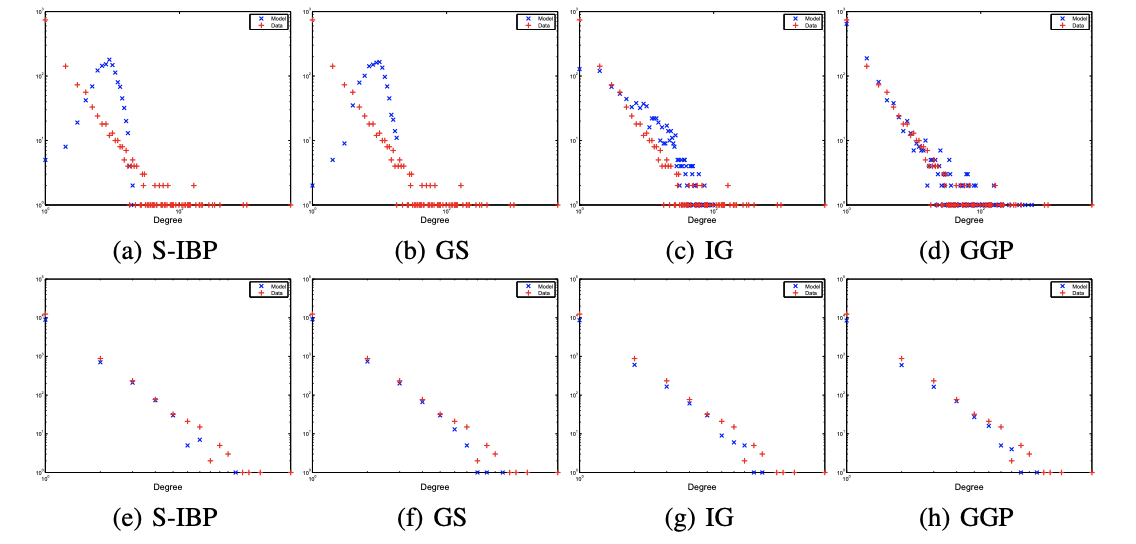
\includegraphics[keepaspectratio, height = 5cm]{utilities/movies_actors.png}
    \caption{Degree distribution  for readers (a-d) and books (e-h) with 4 models: a stable Indian Buffet Process (S-IBP); our model with $\gamma_{i}=\gamma$ and flat prior assigned (GS); our model with $\gamma_{i} \sim \text{Gamma}$ $(a_{\gamma}, a_{\gamma})$ and flat prior assigned to the parameters (IG); our model with GGP prior for $\gamma_{i}$ (GGP). \textcolor{red}{Data are presented in red } and \textcolor{blue}{samples from the models in blue}.}
    \label{fig:movies}
\end{figure}

    
\end{frame}
%------------------------------------------------
\begin{frame}[allowframebreaks]{Bibliography}
\bibliographystyle{alpha}
\nocite{Caron2012BayesianNM, cinlar2011probability, James_Lijoi_Pruenster_2009, kingman_93}
\bibliography{utilities/bibl.bib}
\end{frame}
%----------------------------------------------------------------------------------------

\end{document}